
\documentclass{beamer}
\usepackage[utf8x]{inputenc}

\usetheme{default}
\usepackage{setspace}
\usepackage{hyperref}

\usepackage{listings}
\definecolor{keywords}{RGB}{180,180,0}
\definecolor{comments}{RGB}{60,179,113}
\lstset{
  language=Python,
  frame=lines,
  keywordstyle=\color{keywords},
    commentstyle=\color{comments}\emph
}

\title{A Quick Look At Rpclib}
\author{Burak Arslan}
\usepackage{wasysym}

\hypersetup{
   colorlinks,
   citecolor=blue,
   filecolor=blue,
   linkcolor=blue,
   urlcolor=blue,
   breaklinks=true
}

\begin{document}

\begin{frame}
  \maketitle
\end{frame}

\begin{frame}
  \frametitle{What is Rpclib?}

  \LARGE
\begin{center}

  Rpclib makes it convenient to

  \bigskip

  expose your services using multiple

  \bigskip

  protocols and/or transports.

\end{center}


\end{frame}


\begin{frame}
\LARGE
\begin{center}

  Which seems to be especially important

  \bigskip

  for applications with multiple types of clients

  \large

  \bigskip

  (Native Apps, Browsers, etc.)

\end{center}

\end{frame}

\begin{frame}
\Huge
\begin{center}

  How does it work?

\end{center}

\end{frame}

\begin{frame}[fragile]
  \LARGE
\begin{center}

  Let's start small, with a simple function

  \bigskip

  which we want to be remotely callable:
\end{center}
\end{frame}


\begin{frame}[fragile]
  \large
  \begin{lstlisting}
  from datetime import datetime

  def get_utc_time():
      return datetime.utcnow()
  \end{lstlisting}
\end{frame}

\begin{frame}
  \LARGE

  \color{red} \textbf{1)} \color{black}


    \begin{center}
      We wrap it with Rpclib boilerplate:
    \end{center}

\end{frame}

\begin{frame}[fragile]
  \begin{lstlisting}
  from rpclib.model.primitive import DateTime
  from rpclib.decorator import srpc
  from rpclib.service import ServiceBase

  class DateTimeService(ServiceBase):
      @srpc(_returns=DateTime)
      def get_utc_time():
          return datetime.utcnow()
  \end{lstlisting}
\end{frame}

\begin{frame}
  \LARGE

  \color{red} \textbf{2)} \color{black}

  \begin{center}
    We now wrap the service definition inside

    \bigskip

    an \texttt{Application} definition, where

    \bigskip

    we assign input and output protocols.

  \end{center}

\end{frame}

\begin{frame}[fragile]
  \begin{lstlisting}
from rpclib.application import Application
from rpclib.protocol.http import HttpRpc

httprpc = Application([DateTimeService],
        tns='rpclib.examples.multiprot',
        in_protocol=HttpRpc(),
        out_protocol=HttpRpc()
    )
  \end{lstlisting}
\end{frame}

\begin{frame}
  \LARGE
  \color{red} \textbf{3)} \color{black}

  \begin{center}
    Finally, we wrap the application inside

    \bigskip

    a transport. For this case, we will use

    \bigskip

    the WSGI transport.

  \end{center}

\end{frame}

\begin{frame}[fragile]
 \begin{lstlisting}
from rpclib.server.wsgi import WsgiApplication

application = WsgiApplication(httprpc)
 \end{lstlisting}

  \begin{center}
    This is now a regular WSGI Application that

    \bigskip

    we can pass to wsgi-compliant servers like

    \bigskip

    CherryPy, mod\_wsgi, etc.
  \end{center}
  \pause
  \begin{lstlisting}[language=sh]
$ curl http://localhost:9910/get_utc_time
2012-03-09T17:38:11.997784
  \end{lstlisting}
\end{frame}

\begin{frame}
  \LARGE
  \begin{center}
    Now, what if we wanted to expose this

    \bigskip

    function using other protocols?
  \end{center}
\end{frame}

\begin{frame}[fragile]
  \frametitle{For example: SOAP}

  \begin{lstlisting}
from rpclib.application import Application
from rpclib.protocol.soap import Soap11

soap = Application([DateTimeService],
        tns='rpclib.examples.multiprot',
        in_protocol=HttpRpc(),
        out_protocol=Soap11()
    )
  \end{lstlisting}
\end{frame}

\begin{frame}[fragile]
  \frametitle{For example: SOAP}

  \begin{lstlisting}[language=sh,frame=topline]
$ curl http://localhost:9910/get_utc_time \
                              | tidy -xml -indent
  \end{lstlisting}
  \tiny
  \begin{lstlisting}[language=xml,frame=bottomline]
  <?xml version='1.0' encoding='utf-8'?>
  <senv:Envelope xmlns:wsa="http://schemas.xmlsoap.org/ws/2003/03/addressing"
  xmlns:tns="rpclib.examples.multiple_protocols"
  xmlns:plink="http://schemas.xmlsoap.org/ws/2003/05/partner-link/"
  xmlns:xop="http://www.w3.org/2004/08/xop/include"
  xmlns:senc="http://schemas.xmlsoap.org/soap/encoding/"
  xmlns:s12env="http://www.w3.org/2003/05/soap-envelope/"
  xmlns:s12enc="http://www.w3.org/2003/05/soap-encoding/"
  xmlns:xs="http://www.w3.org/2001/XMLSchema"
  xmlns:wsdl="http://schemas.xmlsoap.org/wsdl/"
  xmlns:xsi="http://www.w3.org/2001/XMLSchema-instance"
  xmlns:senv="http://schemas.xmlsoap.org/soap/envelope/"
  xmlns:soap="http://schemas.xmlsoap.org/wsdl/soap/">
    <senv:Body>
      <tns:get_utc_timeResponse>
        <tns:get_utc_timeResult>
          2012-03-06T17:43:30.894466
        </tns:get_utc_timeResult>
      </tns:get_utc_timeResponse>
    </senv:Body>
  </senv:Envelope>
  \end{lstlisting}
\end{frame}

\begin{frame}[fragile]
  \frametitle{Or, just XML:}

  \begin{lstlisting}
from rpclib.application import Application
from rpclib.protocol.xml import XmlObject

xml = Application([DateTimeService],
        tns='rpclib.examples.multiprot',
        in_protocol=HttpRpc(),
        out_protocol=XmlObject()
    )
  \end{lstlisting}
\end{frame}


\begin{frame}[fragile]
  \frametitle{Or, just XML:}

  \begin{lstlisting}[language=sh,frame=topline]
$ curl http://localhost:9910/get_utc_time \
                              | tidy -xml -indent
  \end{lstlisting}
  \small
  \begin{lstlisting}[language=xml,frame=bottomline]
<?xml version='1.0' encoding='utf-8'?>
<ns0:get_utc_timeResponse
xmlns:ns0="rpclib.examples.multiple_protocols">
  <ns0:get_utc_timeResult>
    2012-03-06T17:49:08.922501
  </ns0:get_utc_timeResult>
</ns0:get_utc_timeResponse>
  \end{lstlisting}
\end{frame}

\begin{frame}[fragile]
  \frametitle{Or, HTML:}

  \begin{lstlisting}
from rpclib.application import Application
from rpclib.protocol.xml import HtmlMicroFormat

html = Application([DateTimeService],
        tns='rpclib.examples.multiprot',
        in_protocol=HttpRpc(),
        out_protocol=HtmlMicroFormat()
    )
  \end{lstlisting}
\end{frame}


\begin{frame}[fragile]
  \frametitle{Or, HTML:}

  \begin{lstlisting}[language=sh,frame=topline]
$ curl http://localhost:9910/get_utc_time \
                              | tidy -xml -indent
  \end{lstlisting}
  \begin{lstlisting}[language=html, frame=bottomline]
<div class="get_utc_timeResponse">
  <div class="get_utc_timeResult">
    2012-03-06T17:52:50.234246
  </div>
</div>
  \end{lstlisting}
\end{frame}


\begin{frame}
  \LARGE
  \begin{center}
    etc...
  \end{center}
\end{frame}

\begin{frame}
  \LARGE
  \begin{center}
    Rpclib also makes it easy to implement

    \bigskip

    custom protocols.
  \end{center}
\end{frame}

\begin{frame}
  \LARGE
  \begin{center}
    Let's implement a protocol that renders

    \bigskip

    the datetime value as an analog clock.

    \bigskip

    \pause
    \large
    (without going into much detail \smiley)

  \end{center}
\end{frame}

\begin{frame}
  \LARGE
  \begin{center}
    To do that, we need to implement the

    \bigskip

    \texttt{serialize} and \texttt{create\_out\_string}

    \bigskip

    functions in a \texttt{ProtocolBase} child.
  \end{center}
\end{frame}

\begin{frame}[fragile]
  \small
  \begin{lstlisting}
from rpclib.protocol import ProtocolBase

class SvgClock(ProtocolBase):
  mime_type = 'image/svg+xml'

  def serialize(self, ctx, message):
    d = ctx.out_object[0] # the return value
    # (some math and boilerplate suppressed)
    # clock is a svg file parsed as lxml Element
    ctx.out_document = clock

  def create_out_string(self, ctx, charset=None):
    ctx.out_string = [
        etree.tostring(ctx.out_document,
            pretty_print=True,
            encoding='UTF-8',
            xml_declaration=True
        )]
  \end{lstlisting}
\end{frame}

\begin{frame}[fragile]
\frametitle{The custom SVG protocol:}
\begin{lstlisting}

from rpclib.application import Application

svg = Application([DateTimeService],
        tns='rpclib.examples.multiprot',
        in_protocol=HttpRpc(),
        out_protocol=SvgClock()
    )

\end{lstlisting}

\end{frame}

\begin{frame}[fragile]
\frametitle{The custom SVG protocol:}

  \begin{lstlisting}[language=sh]
$ curl http://localhost:9910/get_utc_time \
                              > utc_time.svg
  \end{lstlisting}

  \begin{center}
    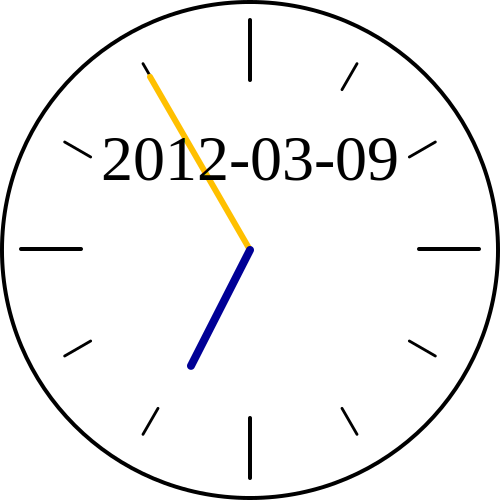
\includegraphics[scale=.4]{get_utc_time.pdf}
  \end{center}
\end{frame}

\begin{frame}
  \huge
  \textbf{So, what's missing?}
  \begin{center}
\Large
  \begin{tabular}{ll}
    \textbf{Protocols}:  & JSON! ProtoBuf! XmlRpc! \\
                         & HTML! (The whole document) \\
    \textbf{Transports}: & SMTP!
  \end{tabular}

  \bigskip

  \large
  $\left(
    \begin{tabular}{c}
    and many other things! see the ROADMAP.rst \\
    in the source repo.
  \end{tabular}
  \right)$

  \end{center}
\end{frame}

\begin{frame}
  \frametitle{Additional Information:}

  \begin{center}
  \huge

  \href{http://github.com/arskom/rpclib}{github.com/arskom/rpclib}

  \bigskip

  \large

  This example and the presentation are in:
  \href{https://github.com/arskom/rpclib/tree/master/examples/multiple_protocols}{examples/multiple\_protocols}

  \bigskip

  \huge

  % If interested, grab me during the
  %
  % \bigskip
  %
  % sprints, I'll be around!

  \end{center}

\end{frame}

\end{document}
